
To communicate with a computer, one is required to ''speak'' the same language as the machine. A computer's language is pre-defined by the manufacturer of the computer, and generally referred to as \emph{machine code} or \emph{machine instructions}.\\
Today's software developers make use of various programming languages and each language deals with an area of functionality. These languages have to be translated for the computer and this is done with tools called compilers.\\
When developing, the choice of programming language can be vital to the project's success and functionality.\\\\
In this report, a description of the development-process of a new language is laid out.

\section{\langname{}}
The purpose of this project is to address the interest for a role-playing based language. With this language it should be possible to define characters, skills, attributes, effects etc, commonly found in \ac{rpgs} and thereafter simulate a battle between characters.

To do this, the language should capture the intuitive and simple characteristics of character sheets. Character sheets can be thought of as information containers for various Role-playing games. They keep track of the character's skill- and health-state as well as inventory. An example of a character-sheet can be found in appendix \vref{charsheet}).

\section{Role-playing}
Role-playing games have been commercially available since the 1970's and exist in various forms. \ac{rpgs} can be described as interactive storytelling, meaning that the players take on the part of characters on the adventure being told. When actions are unrestricted and players are free to do as they please, the scenario becomes more than a story, evolving into an interactive experience between the players and the storyteller, involving social encounters, travelling, fighting and more.

\textbf{For many players the most exciting element of \ac{rpgs} is the fighting and how it is defined and/or simulated.}
\\\\
There are currently three types of \ac{rpgs} available; \emph{Computer-}, \emph{\ac{pnp}-} and \emph{Live Action \ac{rpgs}}, the first two being the focus in this project.

In \ac{rpgs}, players take on the roles of fictitious characters, most often created by the players themselves.
When playing \emph{\ac{pnp}- \ac{rpgs}}, a core rulebook is used, to solve conflicts, get inspiration for adventures, character creation, reference and more. In \emph{Computer- \ac{rpgs}}, the rulebook is replaced by static rules implemented in the game world, however developers often provide useful information (much like rulebooks) for the players in the form of a guide or a codex.

Characters are defined by their abilities and attributes (collectively known as ''stats'', short for statistics), meaning that each ability is assigned a number that represents how ''good'' the character is at using a given ability. This is also the case with attributes and certain ''traits'' (e.g superpowers). An attribute is a value which indicates how much better or worse a character is compared to other beings in the game world. Take for example the attributes \emph{strength} and \emph{charisma}. Strength tells you how strong a character is, often used to measure how much they can lift and how hard they can hit. Charisma is a character's social skill level, used to measure how well they can handle social situations. Most games break as much as possible down to numbers; appearance, intellect, luck and more. This helps balance the characters in relation to their environment.

The first modern \emph{\ac{pnp} \ac{rpg}} to be released commercially was the game \emph{\ac{dnd}}, which was first published in 1974.\cite{wikidnd}
\emph{\ac{dnd}} can therefore be thought of as the pioneer of role-playing games.

\subsection{Character creation}
How a character is created varies from system to system. Common for most is that the characters all have stats describing them.
They can indicate a certain status amongst peers (e.g on a scale of 0 - 10), serve as a counter for how often a certain ability or item can be used, tell a character's level of skill and/or trait (such as Strength) and last but not least they keep track of the character's resources (such as \ac{hp}).
\ac{hp} is a measure for how much damage a character can take before dying. Strength can be used to calculate how much damage a character can do to others. Depending on what stat is in question, it can be decided by rolling dice, be computed from other stats, assigned specifically by the player or based on the player's choices during character creation.

\subsection{Pen \& Paper}
When playing \emph{\ac{pnp}} the players generally use various dice (see figure \ref{dice}) to determine the outcome of an activity, for example an attack, where the dice determines if the attack is successful and thereafter how much damage is inflicted. To help keep track of a character's attributes and other information, a character sheet is used.

In \ac{pnp} games the participants are: A \ac{gm}, who is responsible for control of \ac{npc}s, environment, the setting of the adventure and has the final say in conflicts. The players each control their individual characters, around which the adventure revolves.

A game scenario can be described as following: The \ac{gm} prepares an adventure for the players and lays down additional rules if needed. Participants are seated around a table with their character sheets and a number of dice. Each player has created a character to use in the given adventure. The \ac{gm} describes the setting and series of events, playing all \ac{npc}s. The players roleplay their characters and determine their actions by themselves. When an action is required from a specific player, they can determine the outcome of the action by rolling a set of dice.
\begin{figure}[!h]
\centering
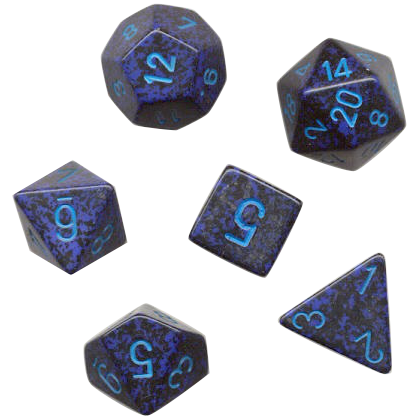
\includegraphics[scale=0.35]{img/rpgdice.png}
\caption{Dice for role-playing purposes}
%\cite{rpgdice}
\label{dice}
\end{figure}

\subsection{Digitised}
In \emph{Computer \ac{rpgs}} the outcome of an activity is determined by measures implemented by the developers. This can be an imitation of a dice roll (variation) or a static calculation (pre-calculated).
To keep track of character information, a digitised character sheet is often accessible, where the player can customise their character to some degree.

In computer \ac{rpgs} the player will often be given a set of possible actions to choose from, and it is up to the player to determine which one suits the situation best. The opponents are pre-programmed to react in a certain way to various events, such as when their health decreases.

\pagebreak

%source: (wikidnd) http://en.wikipedia.org/wiki/History_of_role-playing_games
